\chapter{Range queries in the snapshot model}
\thispagestyle{myheadings}

	A persistent adversary is capable of observing not only the data at any point in time (like the snapshot attacker), but also all processes and communication on the server, including the network messages, their size, and the access pattern to the storage.
	A series of attacks starting with a seminal work of \textcite{generic-attacks-kellaris} showed that the query result size~\cite{generic-attacks-kellaris, state-of-uniform, attacks-improved-reconstruction, pump-volume-attacks, volume-range-attacks} and access pattern~\cite{multidimensional-range-queries, inference-attack-islam-14, leakage-abuse-attacks-cash-15, inference-attacks-naveed-15, generic-attacks-kellaris, attacks-tao-of-inference, grubbs-attacks, access-pattern-disclosure, attacks-improved-reconstruction} alone could enable reconstruction attacks.
	The attacks against the access pattern typically exploit the fact that some records are accessed more often than others and in the same query as others.
	The adversary maps this knowledge to some public auxiliary dataset and queryset, and guesses the values correctly with a non-negligible probability.
	Attacks on communication volume are more elaborate and use the fact that there are a well-defined number of distinct interval queries over the domain.
	\textcite{generic-attacks-kellaris}, for example, construct a polynomial with the observed number of queries that return a different number of records, and solve it deriving the exact reconstruction.

	A generic way to protect the access pattern is the \acrfull{oram}, an interactive client-server protocol that conceals the access pattern from the observing adversary by making at least $\bigO{\log n}$ extra requests.
	A na\"{\i}ve solution is to simply proxy all requests through the \acrshort{oram} protocol, but it is generally inefficient and not trivially parallelizable.

	Protecting against communication volume leakage usually involves returning a number of extra fake records and letting the client filter them out locally.
	Where approaches differ is in the number of these fake records.
	A na\"{\i}ve way of adding a constant amount of noise or even sampling noise uniformly is insecure since such noise can be filtered out by the adversary either immediately (constant noise) or after observing a certain number of queries (uniform noise).
	Another dimension to the problem is how much noise to add to have a provable guarantee and yet add the smallest amount of noise possible.

	\section{Enhanced Outsourced Database model}

		In this work we aim for the most practical definition of security, which needs to capture both access pattern and communication volume protection and yet be feasible enough so that an efficient system exists that can satisfy it.
		In \epsolute{} \cite{epsolute} we propose a definition of computationally \acrshort{dp} outsourced database.

		\begin{definition}[\acrfull{cdpodb} from Definition 3.1 in \cite{epsolute}]\label{definition:cdpodb}
			We say that an outsourced database system \protocol{} is $(\epsilon, \delta)$-computationally differentially private (a.k.a. \acrshort{cdpodb}) if for every polynomial time distinguishing adversary \adversary{}, for every pair of neighboring databases $\database \sim \database^\prime$, and for every query sequence $\fromNtoM{\query}{1}{m} \in \querySet^m$ where $m = \mathsf{poly}(\lambda)$,

			\begin{multline*}
				\probability{\adversary \left( 1^\lambda, \view{\protocol, \server}{\database, \fromNtoM{\query}{1}{m}} \right) = 1 } \leq \\
				\exp{\epsilon} \cdot \probability{\adversary \left( 1^\lambda, \view{\protocol ,\server}{\database^\prime, \fromNtoM{\query}{1}{m}} \right) = 1} + \delta + \negl \; ,
			\end{multline*}
			the probability is over the randomness of the distinguishing adversary \adversary{} and the protocol \protocol{}.
		\end{definition}

		The first thing to note in this definition is that unlike in prior works where only a part of \adversary{}'s view is \acrshort{dp}-protected (e.g., only access pattern in \cite{differential-obliviousness,differential-obliviousness-followup}), here the entire view of the adversary is protected.
		That is, if \emph{anything} visible during the execution of the protocols to a persistent adversary can be used to distinguish the neighboring datasets, the adversary wins and the system fails to satisfy the definition.
		Subsequently, it implies protection against both access pattern and communication volume, since they are both a part of the view and thus if the adversary sees either of them, she can distinguish.

		Also note that the \acrshort{cdpodb} system is \acrshort{dp}, but not necessarily semantically secure.
		A semantically secure database would have had probabilities almost equal (or, in \cref{definition:cdpodb}, $\epsilon = 0$).
		The trade-off has been made to allow construction of an efficient system.
		While a na\"{\i}ve solution that satisfies the semantically secure definition would return the entire dataset every query, constructing a practical instantiation is hard, is not necessarily possible, and remains an open problem.

		The negligible term $\negl$ at the end was added to account for the computational (as opposed to the information-theoretical) nature of the definition.
		In the information-theoretical system the security is guaranteed by the clear mathematical proof that the adversary can do nothing better than brute-force the system (e.g., iterating over one-time-pad keys).
		A computational security definition relies on the fact that the adversary simply does not have enough resources to break a system, which may or may not hold true in the future.
		For example, the problems of finding a discrete logarithm and factorization are only assumed to be hard, as are standardized block ciphers, such as AES \cite{aes-nist}.
		Therefore, if we want to allow a system to use these cryptographic blocks for security, we must include the negligible term in the definition.

		Finally, note the query sequence $\fromNtoM{\query}{1}{m} \in \querySet$ is fixed.
		The definition is non-adaptive meaning that the user \user{} must not choose the next query based on the result of the previous one.
		In \cite[Section 3.1.1]{epsolute} we prove by example why this limitation is inherent and no efficient system can be built that would allow adaptive queries.

	\section{Single-threaded \epsolute{}}

		In \epsolute{} \cite{epsolute}, we develop a method of answering point and range queries that satisfies \cref{definition:cdpodb}.
		At the heart of the construction is the use of \acrshort{oram} to hide the access pattern and \acrshort{dp} to add extra fake records to the result to hide communication volume.

		\acrshort{oram} component is straightforward --- communication between \user{} and \server{} is routed through the \acrshort{oram} protocol.
		This approach, however, substantially increases the overhead, which I will address in \cref{section:range-queries-persistent:parallel-epsolute}.

		To optimally add noise to the true result we make use of sanitizers for point and range query types.
		For point queries, we construct a histogram from the domain values.
		We put the number of records for the domain value plus the noise sampled from the Laplacian distribution into each bin.

		\begin{figure}[h]
	\centering
	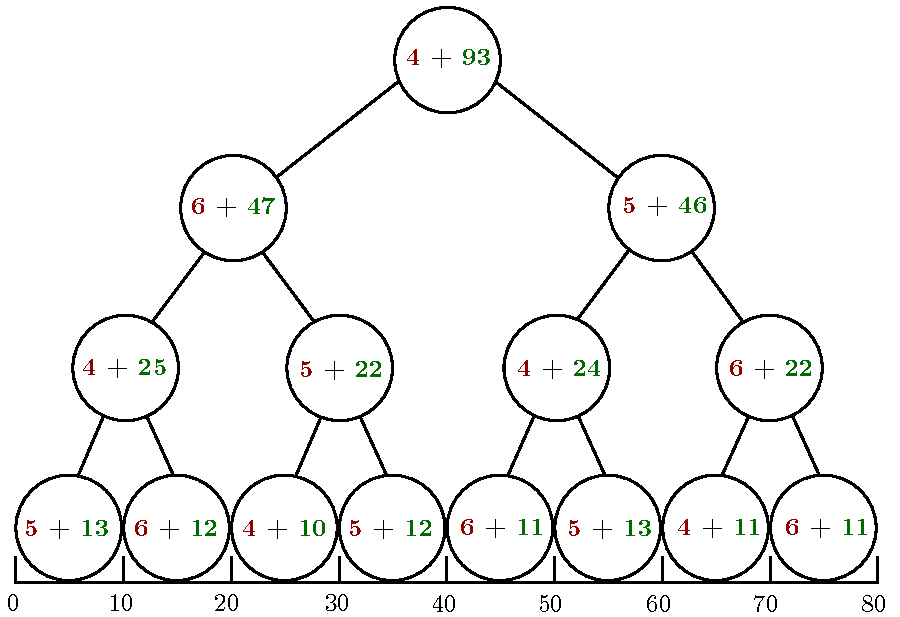
\includegraphics[width=1.0\textwidth]{sanitizer}
	\caption[An example of a hierarchical sanitizer]{
		An example of a hierarchical sanitizer \cite{hierarchical-methods-for-dp} with fanout $\fanout = 2$.
		Left (red) value is noise and right (green) value is the number of records covered by the node.
		To answer a query $[3, 28]$, we take only two nodes $(4 + 25)$ and $(4 + 10)$ with a resulting noise of 8 and 35 real records.
	}\label{figure:sanitizer}
\end{figure}


		For the range queries we use a hierarchical sanitizer \cite{hierarchical-methods-for-dp}, see example in \cref{figure:sanitizer}.
		We first split the continuous domain into bins.
		Then we build a \fanout{}-ary tree over domain bins and put the number of records plus noise into each node.
		The leaves get values the same way as in histogram, and intermediate node value is a sum of counts of all records in all children bins plus a single noise sample.
		Compared to a plain histogram, this construction has the benefit that if the range is wide we can answer the query using only the intermediate node and not all leaf nodes.
		Since each bin is now associated with $\ceil{\log_\fanout B}$ nodes, where $B$ is the number of bins, we amplify our noise respectively.

		Note that the Laplacian distribution is symmetrical and unbounded, so if we sample from a zero-mean distribution some of the samples will be negative.
		Since we do not allow negative noise and since na\"{\i}vely truncating the distribution will break \acrshort{dp} guarantees, we need to shift the mean of the distribution.
		Doing so will only increase the noise thereby maintaining the guarantees.
		We have analytically derived the smallest mean of the distribution to ensure that the samples are non-negative for the entire histogram or tree with a set probability $\delta$.
		These values are
		\[
			\mu_{\mathsf{point}} = \ceil{ -\frac{ \ln \left( 2 - 2 \sqrt[\domainSize]{1 - \delta} \right) }{ \epsilon } } \quad \text{and} \quad \mu_{\mathsf{range}} = \ceil{ -\frac{ \ln{ (2 - 2 \sqrt[\mathsf{nodes}]{ 1 - \delta } ) } \cdot \log_{\fanout} \domainSize }{\epsilon} }
		\]
		for domain size \domainSize{} and the number of nodes in a tree $\mathsf{nodes}$.

		With these prerequisites we construct the actual setup and query protocols.
		See the visualization of \protocolQuery{} in \cref{figure:epsolute}.
		\begin{itemize}
			\item
				Setup protocol \protocolSetup{}
				\begin{enumerate}
					\item
						On input a dataset \database{}, \user{} creates and keeps locally an inverted index over the records mapping the search keys \searchKey{} to record IDs \recordID{}.
					\item
						\user{} and \server{} engage in the \acrshort{oram} protocol, where \user{} is a client.
						\user{} stores all records by their IDs.
					\item
						\user{} constructs a sanitized structure \serverDS{}, a \acrshort{dp}-histogram for point queries or a \acrshort{dp}-tree for range queries, over the dataset domain and posts it to \server{}.
				\end{enumerate}
			\item
				Query protocol \protocolQuery{}
				\begin{enumerate}
					\item
						On input a query \query{}, \user{} looks up record IDs in its local index.
					\item
						\user{} requests \serverDS{} from \server{} and uses it to calculate the total number of requests $c$ (the number of true records for the query plus noise).
					\item
						\user{} and \server{} engage in the \acrshort{oram} protocol, where \user{} is a client.
						\user{} loads $c$ records where these requests include all true records and the rest are random and non-repeating.
					\item
						\user{} prunes the fake records and returns the true ones.
				\end{enumerate}
		\end{itemize}

		\begin{figure}[h]
	\centering
	\includegraphics[width=1.0\textwidth]{epsolute}
	\caption{Query protocol \protocolQuery{} of \epsolute{}.}\label{figure:epsolute}
\end{figure}


		This method, to which I will refer to as \emph{a single-threaded \epsolute{}}, is a \acrlong{cdpodb} as defined in \cref{definition:cdpodb}, see proof in \cite[Section 4.2]{epsolute}.

	\section{Parallel \epsolute{}}

		While the single-threaded \epsolute{} is an efficient \acrshort{cdpodb} in the sense that it returns only a fraction of total records per query, it is still slow in practice because of the $\bigO{\log \dataSize \log \domainSize}$ overhead due to \acrshort{oram} and \acrshort{dp}-sanitizer.
		To bring the construction closer to real-world demands in performance we devise a parallel solution.

		\subsection{A choice of separate vs shared sanitized dataset}

			A natural approach is to split the dataset \database{} into \oramsNumber{} partitions and run parallel \acrshort{oram} protocols against a distributed \server{}.
			The partitioning part is not hard --- we split records by the hash of their unique ID and construct smaller (and thus logarithmically faster) \acrshortpl{oram} over the partitions along with \oramsNumber{} inverted indices on \user{}.
			However, we need to decide how we sample \acrshort{dp} noise in this setting.
			The two approaches are generating a separate \serverDS{} per partition or using a shared \serverDS{}.

			When generating a separate \acrshort{dp}-sanitized dataset \serverDS{} per partition there are two competing effects on performance.
			On the one hand, each thread on average returns a \nicefrac{1}{m} fraction of the result from an \acrshort{oram} with overhead $\log \frac{n}{m}$.
			On the other hand, each thread now adds independent noise, which results in \oramsNumber{} times amplification of noise.
			Moreover, due to the \acrshort{dp} composition theorem \cite{privacy-integrated-queries,differential-privacy-original,our-data-ourselves} for disjoint datasets, the privacy budget of the system is the privacy budget of the least private component.
			Since we cannot assume that the distribution of resulting records in all queries is always uniform, we bound a worst-case scenario of a single \acrshort{oram} having most of the result records.
			In \cite[Section 5.1]{epsolute} we have found that the noise is amplified by an extra $\left( 1 + \sqrt{ \frac{-3 m \log \delta}{k_0} } \right)$ factor, where $k_0$ is the number of true records for a query.

			When generating a single shared \serverDS{} for all \oramsNumber{} partitions, we need to ensure that the total number of records returned by each thread is the same.
			We reuse the amplification factor from previous approach and set new $\tilde{k}_0 = k_0 + \frac{\log^{1.5} N}{\epsilon}$ for range queries and $\tilde{k}_0 = k_0 + \frac{\log N}{\epsilon}$ for point queries due to the use of \acrshort{dp} sanitizers.
			The total generated noise is now larger but it is now split among \oramsNumber{} threads and it grows slower than linear in \oramsNumber{}.

			Comparing these two methods we conclude that in most cases the shared \serverDS{} is faster (i.e., results in fewer total fetched records), especially for an increasing parallelization factor.
			First, the former method is not guaranteed to have a uniform load among threads.
			In fact, while on average the amount of work per thread may be smaller, there may be a single disproportionally overloaded thread, which would cause the entire system to slow down.
			Second, while the number of true records per thread will decrease linearly for the former method, the noise factor will stay constant and will at larger \oramsNumber{} dominate the amount of work precluding further scalability.
			The latter method is more scalable in this regard since the amount of work decreases linearly while the amount of noise increases only logarithmically with the number of threads.

		\subsection{The construction}

			With this analysis I present an upgraded construction, \emph{a parallel \epsolute{}}, see \cref{figure:parallel-epsolute}.
			The core protocol is similar to the single-threaded version except some of the operations are distributed and executed in parallel.
			\begin{itemize}
				\item
					Setup protocol \protocolSetup{}
					\begin{enumerate}
						\item
							On input a dataset \database{}, \user{} partitions it into \oramsNumber{} segments \fromNtoM{\database}{1}{\oramsNumber} by a hash of record IDs \recordID{}.
							\user{} then creates and keeps locally \oramsNumber{} inverted indices over the records mapping the search keys \searchKey{} to record IDs \recordID{} in a respective partition.
						\item
							\user{} and distributed \server{} engage into \oramsNumber{} \acrshort{oram} protocols, where \user{} is a client.
							\user{} stores all records by their IDs in respective \server{} partitions.
						\item
							\user{} constructs a sanitized structure \serverDS{} (or \oramsNumber{} such structures depending on the choice of method) over the domain of the dataset and posts it to \server{}.
					\end{enumerate}
				\item
					Query protocol \protocolQuery{}
					\begin{enumerate}
						\item
							On input a query \query{}, \user{} looks up record IDs in its local indices.
						\item
							\user{} requests (one or multiple) \serverDS{} from \server{} and uses it to calculate the total number of requests $c$.
							Depending on the choice of method, \user{} prepares a sequence of requests to \server{}.
						\item
							\user{} and \server{} engage into \oramsNumber{} \acrshort{oram} protocols, where \user{} is a client.
							\user{} loads a total of $c$ records where these requests include all true records and the rest are random and non-repeating.
						\item
							\user{} waits for the last thread to finish, prunes the fake records and returns the true ones.
					\end{enumerate}
			\end{itemize}

			As a purely practical optimization, instead of making a single client \acrshort{vm} engage into \oramsNumber{} (up to 128 in the experiments) connections and heavy cryptographic threads, we logically split \user{} into a principal \acrshort{vm}, which handles main logic, and a set of helper \acrshortpl{vm} that only engage in a number of \acrshort{oram} protocols.

			\begin{figure}[th]
	\centering
	\includegraphics[width=1.0\textwidth]{parallel-epsolute}
	\caption{Query protocol \protocolQuery{} of parallel \epsolute{}.}\label{figure:parallel-epsolute}
\end{figure}


	\section{Experimental Evaluation}

		To empirically verify the efficiency and practicality of our solution, we have implemented the construction in C++ \cite{github-epsolute} and have run an extensive set of experiments.
		We have designed the experiments to
		\begin{enumerate*}[label=(\alph*)] % chktex 36
			\item compare our system to competing proposed systems,
			\item measure the storage overhead,
			\item tune the parameters of the system and observe the effect on performance,
			\item see how the system scales,
			\item understand the quantitative impact of our optimizations, and
			\item measure the impact of supporting multiple attributes.
		\end{enumerate*}

		For the default setting we ran range queries in the parallel \epsolute{} using the shared \serverDS{} method.
		Client \acrshort{vm} managed $\oramsNumber = 64$ threads, which are split among 8 lightweight \acrshort{oram} \acrshortpl{vm}.
		Client \user{} and server \server{} are located in geographically distributed regions, with the ping time between the regions \SI{12}{\milli\second} and the effective bandwidth \SI{150}{\mega\byte\per\second}.
		In this section I will focus on comparing \epsolute{} to relevant systems and on \epsolute{}'s scalability.
		I refer to the full work for the rest of the experimental findings \cite[Section 6]{epsolute}.

		\subsection{Against relevant solutions}

			In \cite{epsolute}, we compared \epsolute{}
			\begin{enumerate*}[label=(\alph*)] % chktex 36
				\item to conventional \acrshort{sql} \acrshortpl{rdbms} (PostgreSQL and MySQL),
				\item to a linear scan approach, and
				\item to Shrinkwrap \cite{shrinkwrap}.
			\end{enumerate*}

			\acrshortpl{rdbms} are highly optimized for range queries --- the records indexed by search keys are typically stored continuously in-order and the database streams back these blocks very efficiently.
			As a baseline approach, \acrshortpl{rdbms} were configured for maximum performance and minimum security.

			Linear scan is a strawman approach, which downloads the entire encrypted dataset every query, decrypts it and then runs the query locally.
			This is the opposite baseline of maximum security and poorest performance.
			Such an approach is not entirely theoretical: some commercial \acrshortpl{rdbms} exhibit linear scan behavior when configured for maximum security, for example MS-SQL Always Encrypted with Randomized Encryption \cite{mssql-always-enc} and Oracle Column Transparent Data Encryption \cite{oracle-tde}.

			Shrinkwrap \cite{shrinkwrap} is a construction that executes federated \acrshort{sql} queries securely, albeit inefficiently.
			To hide communication volume it fully pads the intermediate results of the sub-queries (although it ``shrinks'' the output before passing it to the next stage).
			To hide the access pattern, the algorithm makes a linear scan over the entire input.
			Moreover, to process the encrypted data (e.g., evaluate a predicate), the whole program is compiled into garbled circuits \cite{yao-circuits,emp-toolkit}.

			\begin{figure}[!ht]
	\centering
	\includegraphics[width=\textwidth]{mechanisms}
	\caption[Different range-query mechanisms]{
		Different range-query mechanisms (log scale).
		Default setting: $10^6$ \SI{4}{\kibi\byte} uniformly-sampled records with the range $10^4$.
	}%
	\label{figure:mechanisms}
\end{figure}


			We conclude that \epsolute{} is efficient --- while answering a query in \SI{840}{\milli\second}, it is only 8 to 4 times slower than a typical \acrlong{rdbms}, 18 times faster than the scan, and three orders of magnitude faster than the Shrinkwrap, see \cref{figure:mechanisms}.

		\subsection{Scalability}

			To measure scalability we have run parallel \epsolute{} with shared and separate \acrshort{dp}-sanitized datasets \serverDS{} for a varying number of threads \oramsNumber{}.
			For a truly scalable system we would observe a drop in overhead roughly proportional to the increase in parallelization factor \oramsNumber{}.
			We confirm experimentally that \epsolute{} is scalable when a shared \serverDS{} is used as a method of noise generation, see \cref{figure:scalability}.
			The noise dominates the performance of the separate \serverDS{} method for a higher number of threads, while the shared \serverDS{} method continues to scale.

			\begin{figure}[!ht]
	\centering
	\includegraphics[width=\linewidth]{scalability}
	\caption{Scalability measurements for \protocolGamma{} and \protocolNoGamma{}}%
	\label{figure:scalability}
\end{figure}

